\section{Introduction}
\label{sec:intro}

This paper is about the semantic structures underlying probabilistic
programming with random graphs. Random graphs have applications in
statistical modelling across biology, chemistry, epidemiology, and so
on, as well as theoretical interest in graph theory and combinatorics (e.g.~\cite{graphs-handbook}). Probabilistic programming, i.e.~programming for statistical
modelling~\cite{probprog-intro}, is useful for building the statistical
models for the applications. Moreover, as we show
(Theorem~\ref{thm:eq-theory-to-graphon} and Corollary~\ref{corollary:graphon-markov}),
%and~\ref{thm:syntactic-completeness}), 
the semantic aspects of programming languages for random graphs
correspond to graphons~\cite{MR3012035}, a core structure in graph
theory and combinatorics. 


To set the scene more precisely, we recall the setting of
probabilistic programming with real-valued distributions, 
and contrast it with the setting with graphs.
Many probabilistic programming languages provide a type of
real numbers ($\treal$) and distributions such as the normal
distribution
\begin{equation}\label{eqn:tnormal}
  \tnormal :\treal\ast\treal\to \treal
\end{equation}
together with arithmetic operations such as
\begin{equation}\label{eqn:add}
  (+) :\treal\ast\treal\to \treal\text.
\end{equation}
Even if we encounter an unfamiliar distribution over $(\treal)$ in a library, we have
a rough idea of how to explain what it could be, in terms of probability
densities and measures.

In this paper, we consider the setting of probabilistic programming with graphs, where
the probabilistic programming language or library provides a type $(\tvertex)$ and some distribution 
\begin{equation}\label{eqn:intro-new}
  \tnew : \tunit \to \tvertex
\end{equation}
together with a test
\begin{equation}\label{eqn:intro-edge}
  \tedge:\tvertex\ast\tvertex\to \tbool\text.
\end{equation}
Our goal is to analyze the interface $(\tvertex,\tnew,\tedge)$ for graphs semantically,
and answer, for instance, what they could be and what they could do. We give one example analysis in Section~\ref{sec:intro:graphs} first, and the general one later in Theorem~\ref{thm:eq-theory-to-graphon} and Corollary~\ref{corollary:graphon-markov}, which says that to give an implementation of
$(\tvertex,\tnew,\tedge)$, satisfying the laws of probabilistic
programming, is to give a graphon. In doing so, we connect 
the theory of probabilistic programming with graph theory and
combinatorics.

Probabilistic programming is generally used for statistical inference, in which we describe a generative model by
writing a program using primitives such as \eqref{eqn:tnormal}--\eqref{eqn:intro-edge} above, and then infer a distribution on certain parameters, given particular observed data.  This paper is focused on the generative model aspect, and not inference (although for simple examples, generic inference methods apply immediately, see~\S\ref{sec:intro:practice}). 

\subsection{Example of an Implementation of a Random Graph: Geometric Random Graphs}
\label{sec:intro:graphs}

To illustrate the interface $(\tvertex,\tnew,\tedge)$ of
\eqref{eqn:intro-new}--\eqref{eqn:intro-edge},
we consider for illustration a random geometric graph (e.g.~\cite{penrose-rgg,https://doi.org/10.1002/rsa.20633}) where the vertices are
points on the surface of the unit sphere, chosen uniformly at random, and where there is an
edge between two vertices if the angle between them is less than
some fixed~$\theta$.
%See Figure~\ref{fig:graph} for samples from such a random
%graph, where  $θ ≝ π/3, \; π/6$.
This random graph might be used, for instance, to model the connections between people on the earth.

For example, a simple statistical inference problem might start from the observed connectivity in Figure~\ref{fig:graph}(a). 
We might ask for the distribution on $\theta$ given that this graph arose from the spherical random geometric graph. One sample from this posterior distribution on random geometric graphs with $\theta=\pi/3$ is shown in Figure~\ref{fig:graph}(b). Another, unconditioned sample from the random geometric graph with $\theta=\pi/6$ is shown in Figure~\ref{fig:graph}(c).  
%Suppose we know this is 
%Although we will not study inference in this paper, we note that one next step for a statistician might
%involve inferring the most likely $\theta$ given particular data. 
%In this paper, rather than inference, we focus on the methods for
%building probability
%distributions.

We can regard this example as an implementation of the interface
$(\tvertex,\tnew,\tedge)$ as follows:
we implement $(\tvertex)$ as the surface of the sphere (e.g. implemented
as Euclidean coordinates). 
\begin{itemize}
\item $\tnew():\tvertex$ randomly picks a new vertex
  as a point on the sphere uniformly at random.
  Figure~\ref{fig:graph}(c) shows the progress after calling $\tnew()$ 15
  times.
\item $\tedge:\tvertex\ast \tvertex \to \tbool$ checks whether there
  is an edge between two vertices; this amounts to checking whether the angle between two points is less than $\theta$. 
  \end{itemize}
\begin{figure}\centering
  % \includegraphics[scale=0.2]{sphere.png}
  %\vspace{-10mm}
(a)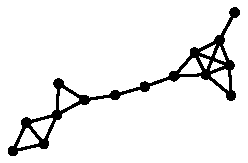
\includegraphics[scale=1,angle=110,valign=t]{graph-data.pdf} \quad (b)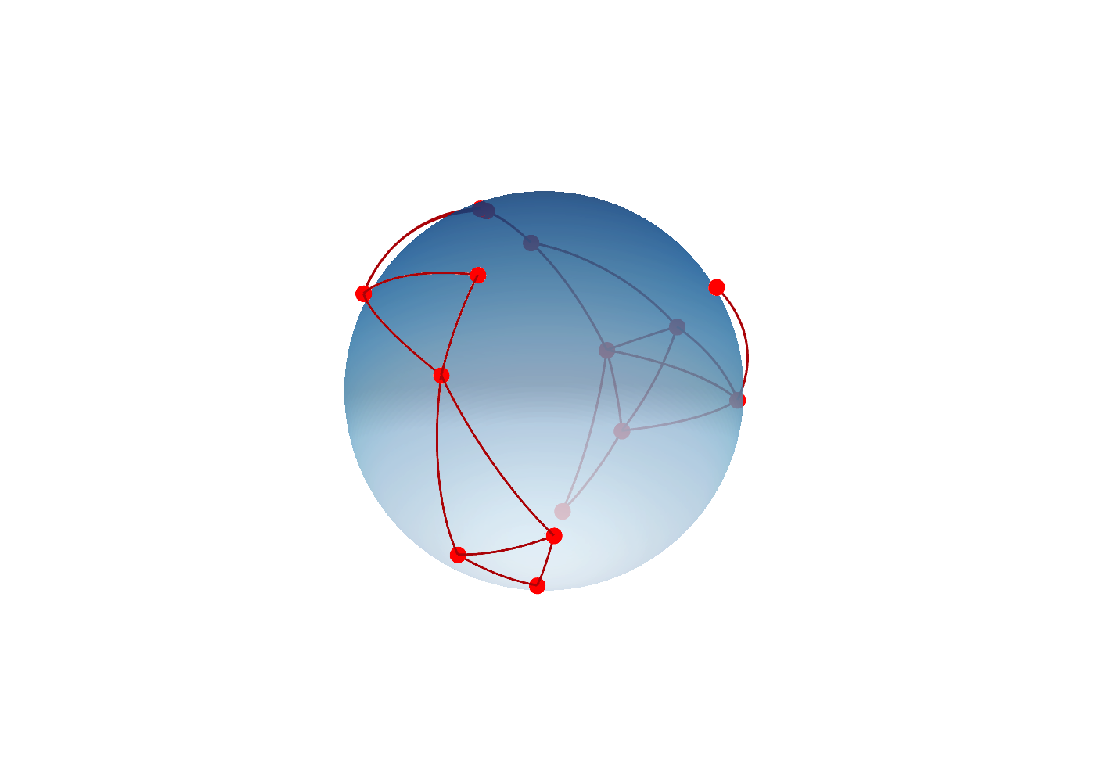
\includegraphics[scale=.5,valign=t]{random-geometric-graph-pi-3_1.pdf} \quad
(c)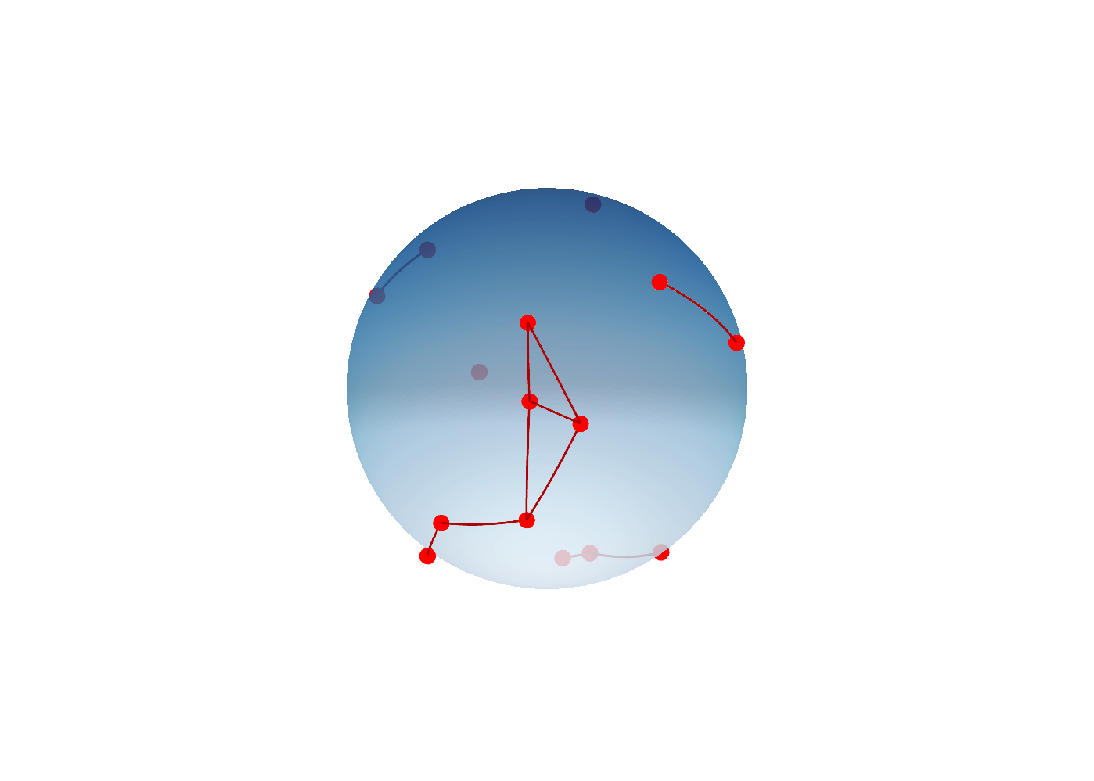
\includegraphics[scale=.5,valign=t]{random-geometric-graph-pi-6_1.pdf}
  \vspace{-1cm}
\caption{(a)~A graph; (b)~an inferred geometric realization of it ($θ \approx π/3$); (c)~a generated sample for $θ = π/6$.\label{fig:graph}}
\end{figure}
For a simple example, we can write a program over the interface to calculate the probability of three
  random vertices forming a triangle: the program
\begin{equation}\label{eqn:triangle}\begin{aligned}&\letin a{\tnew()}{\letin b{\tnew()}{\letin c {\tnew()}
    {}}}\\&\qquad\tedge(a,b) \,\&\, \tedge(b,c) \,\&\,\tedge (a,c):\tbool\end{aligned}
\end{equation}
randomly returns true or false; the probability of true is the
probability of a triangle. 
%(See~\ref{sec:relatedwork} for more practical aspects of programming in this style.)

This implementation using the sphere is only one way to implement
$(\tvertex,\tnew,\tedge)$. There are
implementations using higher-dimensional spheres, or other geometric
objects. We can also consider random equivalence relations as
graphs, i.e.~disjoint unions of complete graphs, or random bipartite
graphs, which are triangle-free. We can consider the
\ErdosRenyi\ random graph, where the chance of an edge between two
vertices is independent of the other edges, and has a fixed
probability.
These are all different implementations of the same abstract
interface, $(\tvertex,\tnew,\tedge)$,
and programs such as \eqref{eqn:triangle} make sense for all of them. 
The point of this paper is to characterize all these
implementations, as graphons. 

\subsection{Implementations Regarded as Equational Theories}\label{sec:intro:eqthys}
The key method of this paper is to treat implementations of the
interface ($\tvertex,\tnew,\tedge$) extensionally, as equational
theories. That is, rather than looking at specific implementation
details, we look at the equations between programs that a user of the
implementation would rely on. (This is analogous to the idea in model
theory of studying first-order theories rather than specific models;
similar ideas arise in the algebraic theory of computational
effects~\cite{pp-notions}.) 
For example, if an implementation always provides a
bipartite random graph, we have the equation 
\[\text{Program~\eqref{eqn:triangle}} \ \ \equiv\ \ \tfalse \qquad\text{between programs,}\]
because a triangle is never generated. This equation does not hold in the example of Figure~\ref{fig:graph}(b--c), since
triangles are possible. 

We focus on a class of equational theories that are well behaved, as
follows.
First, we suppose that they contain basic laws for
probabilistic programming
(eqns.~(\ref{eq:let-assoc})\,--\,(\ref{cd:let_val}), \S\ref{sec:markov-cats}). This basic structure
already appears
broadly in
different guises, including in Moggi's monadic metalanguage~\cite{moggi-computational-lambda}, in linear
logic~\cite{prob-cbpv}, and in synthetic
probability theory~\cite{fritz}. Second, we suppose that the equational theories 
are equipped with a `Bernoulli base', which means that although we do not specify an implementation for the type $(\tvertex)$, each closed program of
type $(\tbool)$ is equated with some ordinary Bernoulli distribution, in such a way as to satisfy the classical laws of traditional finite probability
theory (\S~\ref{sec:bernoulli-base}).
Finally, we suppose that the edge relation is symmetric (the graphs are
undirected) and that it doesn't change when the same question is asked
multiple times (`deterministic'), e.g.
\begin{equation}\letin a{\tnew()}{\letin
                                b{\tnew()}{\tedge(a,b) \,\&\, \neg
                                \tedge(a,b)}}\ \  \ \equiv\ \ \ \ \tfalse \text. \label{eqn:intro:det}\end{equation}

A \emph{graphon} is a symmetric measurable function ${[0,1]^2\to
  [0,1]}$. We show
that every equational theory for the interface
$(\tvertex,\tnew,\tedge)$ gives rise to a graphon (Theorem~\ref{thm:eq-theory-to-graphon}), and conversely that
every graphon arises in this way
(Corollary~\ref{corollary:graphon-markov}).

We emphasize that this abstract treatment of implementations, in terms
of equational theories, is very open-ended, and permits a diverse range of implementation
methods. Indeed, we show in Section~\ref{sec:randomfree} that any
implementation using traditional measure-theoretic methods will
only produce black-and-white graphons, so this abstract treatment is crucial. 

\subsection{From Equational Theories to Graphons}
\label{sec:intro:equations-to-graphons}


In Section~\ref{sec:prog-eq-to-graphons}, we show how an equational
theory over programs in the interface $(\tvertex,\tnew,\tedge)$ gives rise to  a graphon.
The key first step is that graphons (modulo equivalence) can be
characterized in terms of sequences of finite random graphs that
satisfy three conditions: exchangeability, consistency, and locality.

To define a graphon, we show how to define programs that describe finite random graphs, by using
$\tnew$ and $\tedge$ to build boolean-valued $n\times n$ adjacency
matrices, for all $n$ (shown in~\eqref{eqn:programgraph}).
Assuming that the equational theory of programs is Bernoulli-based,
these programs can be interpreted as probability distributions on the
finite spaces of adjacency matrices which, we show, are finite random graphs.  

It remains to show that the induced sequence of random graphs
satisfies the three conditions for graphons (exchangeability,
consistency, and locality). These can be formulated as equational
properties, and so they can be verified by using the equational
reasoning in the equational theory. This is Theorem~\ref{thm:eq-theory-to-graphon}.
A key part of the proof is the observation that exchangeability for graphons
connects to commutativity of $\mathsf{let}$~\eqref{eq:let-comm}: we can permute the order in which
vertices are instantiated without changing the distributions. 


\subsection{From Graphons to Equational Theories}
\label{sec:intro:graphons-to-equations}
We also show the converse: every graphon arises from a good
equational theory for the interface $(\tvertex,\tnew,\tedge)$.
We look at this from three angles: first, we prove this in the general
case using an abstract method, and then, we use concrete methods for
two special cases.

Fixing a graphon, we build an equational theory by following a
categorical viewpoint. A good equational theory for probabilistic
programming amounts to a `distributive Markov category', which is a
monoidal category with coproducts that is well-suited to probability
(\S\ref{sec:markov-cats} and \cite{fritz}). The idea that distributive categories
are a good way to analyze abstract interfaces goes back at least
to~\cite{walters}, which used distributive categories to study
interfaces for stacks and storage. 
We can thus use now-standard abstract methods for building monoidal and
distributive categories to build an equational theory for the
programming language.

We proceed in two steps. We first use methods such as~\cite{hermida-tennent,hu-tholen}
to build an abstract distributive
Markov category that supports the interface
$(\tvertex,\tnew,\tedge)$ in a generic way. This equational theory is
generic and not Bernoulli-based: although it satisfies the equational laws of
probabilistic programming, there is no given connection to traditional probability.
The second step is to  show that (a)~it is possible to quotient this generic category
to get Bernoulli-based equational theories; (b)~the choices of
quotient are actually in bijective correspondence with graphons.
Thus, we can build an equational theory from which any given graphon arises,
via~\eqref{eqn:programgraph}: this is Corollary~\ref{corollary:graphon-markov}.
(The framework of Bernoulli-based Markov categories is new here, and the techniques of~\cite{hermida-tennent,hu-tholen}  have not previously been applied in categorical probability, so
a challenge for future work is to investigate these ideas in other aspects of categorical probability.)

Although this is a general method,
it is an abstract method involving quotient constructions. 
The ideal form of denotational semantics is to explain what programs are by regarding them as
functions between certain kinds of spaces. Although Corollary~\ref{corollary:graphon-markov} demonstrates
that every graphon arises from an equational theory, the type
$(\tvertex)$ is interpreted as an object of an abstract category, and
programs are equivalence classes of abstract morphisms.
In the remainder of the paper, we give two situations where we can
interpret $(\tvertex)$ as a genuine concrete space, and programs are
functions or distributions on spaces. Such an interpretation
immediately yields an equational theory, where two programs are
equal if they have the same interpretation.

\begin{itemize}
\item \emph{Section~\ref{sec:randomfree}}: For `black-and-white graphons', we present 
  measure-theoretic models of the interface, based on a standard
  measure-theoretic interpretation of probabilistic programming
  (e.g.~\cite{Kozen81}).
  We interpret $(\tvertex)$ as a measurable space, and $(\tnew)$ as a
  probability measure on it, and $(\tedge)$ in terms of a measurable predicate. 
  Then, the composition of programs is defined in terms of probability
  kernels and Lebesgue integration.
  This kind of model exactly captures the black-and-white graphons (Prop.~\ref{prop:all-bw}).
\item \emph{Section~\ref{sec:ER-Rado}}: For `\ErdosRenyi' graphons, which are
  constantly gray, and not
  black-and-white, we present a model based on Rado-nominal sets (\S\ref{sec:rado-def}).
  These are a variant of nominal sets (\cite{gp-nominal,pitts-nom-book}) %, already considered in \cite{lmcs:1157},
  where the atoms are vertices of
  the Rado graph (following~\cite{lmcs:1157}). We consider a new notion of `internal
  probability measure' in this setting, and use this to give a 
  compositional semantics that gives rise to the \ErdosRenyi\
  graphons (Corollary~\ref{cor:e-r}).
\end{itemize}
Together, these more concrete sections then provide further intuition for the
correspondence between equational theories and graphons. 

\subsection{Connection to Practice}\label{sec:intro:practice}
We conclude this introduction with remarks on the connection to practical modelling. 
In practice, the graph interface might form part of a generative model, on which we perform inference.
%An instance of the graph interface might depend on certain parameters, such as $\theta$ in the geometric model.
The structure is clearest in a typed language, and one example is the LazyPPL library for Haskell~\cite{lazyppl}.
(Similar examples are implemented in~\cite[Ch.~12]{probmods1},
%http://v1.probmods.org/non-parametric-models.html#example-the-infinite-relational-model
 albeit untyped.)
Then our interface is captured by a Haskell type class:\footnote{See \url{https://lazyppl-team.github.io/GraphDemo.html} for full details in literate Haskell.}
\begin{lstlisting}
class RandomGraph p vertex | p -> vertex where
  new :: p -> Prob vertex
  edge :: p -> vertex -> vertex -> Bool
  \end{lstlisting}
Here \lstinline|p| is a parameter type, and we write \lstinline|Prob| for a probability monad. 
A spherical implementation of the interface (following \S\ref{sec:intro:graphs}) is parameterized by the dimension~$d$ and the distance $\theta$, as follows:
\begin{lstlisting}
data SphGrph = SG Int Double -- parameters for a sphere graph
data SphVertex = SV [Double] -- vertices are Euclidean coordinates
instance RandomGraph SphGrph SphVertex where
  new :: SphGrph -> Prob SphVertex
  new (SG d theta) = ... -- sample a random unit d-vector uniformly 
  edge :: SphGrph -> SphVertex -> SphVertex -> Bool
  edge (SG d theta) v w = ... -- check whether arccos(v.w) < theta
\end{lstlisting}
We can use this as a building block for more complex models.
For a simple example, we generated Figure~\ref{fig:graph}(b) by using the generic Metropolis-Hastings inference of the LazyPPL library to infer $\theta$ given a particular graph (Fig.~1(a)). We have also implemented other random graphs; our implementation of the \ErdosRenyi\ graph uses stochastic memoization~\cite{roy2008stochastic,kaddar-staton-stoch-mem}.


\subsubsection*{Summary and context}
As we have discussed, our main result is that equational theories for the programming interface (\S\ref{sec:intro:graphs})
give rise to graphons (\S\ref{sec:intro:equations-to-graphons}) and every graphon arises in this way~(\S\ref{sec:intro:graphons-to-equations}).

These results open up new ways to study random graphs, by using programming semantics. On the other hand, our results here put the abstractions of practical probabilistic programming on a solid theoretical foundation (see also~\S\ref{sec:relatedwork}).


\hide{
\paragraph*{Related work and summary}
The relationships between graphons, programming, and computability are
well explored -- see Section~\ref{sec:relatedwork} for further discussion.
In this paper we explore a new relationship between graphons and
equational theories of graph programming languages. \todo{This last
  sentence is a bit weak.}}

\hide{\subsection{Informal notes}
{\it
Informal summary of the narrative, to be threaded throughout.

\begin{itemize}
\item \S2: We give a language for building generative models over
  graphs. Some little examples ought to motivate, either in the intro
  or in the text. I think graphs over spheres could be good for
  illustrations.

  We are interested in equational reasoning about programs.
  Although the equational theory ought to have some basic
  properties, the exact equational theory is not fixed.

  The point of the paper is to show that to pick an equational theory
is to give a graphon. 
\item \S3: We show how every choice of equational theory gives a
  graphon.
\item \S4: We show how every graphon arises in this way. Thus
  everything is complete.

  The equational theory here is
  derived via syntactic means and not by saying that programs are
  equal in some mathematical model.
  This makes it very difficult to calculate or have an intuition for
  program fragments. So we seek a denotational
  interpretation of the types of this language.
  And we will do this in two instances.
\item \S5: We give a denotational measure-theoretic interpretation for black-and-white
  graphons.
\item \S7: We give a denotational interpretation for \ErdosRenyi graphons, in
  terms of measures on the vertices of the Rado graph. Basics of this
  are currently in \S6.
  \end{itemize}
  }}
%%% Local Variables:
%%% mode: latex
%%% TeX-master: "popl24"
%%% End:
